\subsection{Spline Interpolation}
There are \textbf{four} main drawbacks of polynomial interpretation.
\begin{enumerate}
    \item On uniformly-spaced points (e.g., data collected over time intervals), higher-order interpolation leads to unbounded oscillations
    \item Special data is needed to interpolate using the Chebyshev method
    \item We have a lack of control and accuracy of the error,
    \[\left|f(x)-f_n(x)\right| \leq C_n h^n\]
    since $C_n$ depends on $f^{(n)}$ on $[a, b]$ and may grow for large $n$
    \item Changing one data point affects the interpolant globally
\end{enumerate}
The solution to these drawbacks is to use \textbf{splines}. Formally,
\begin{defn}[Spline]
    Consider a set of points $\left\{\left(x_i, y_i\right)\right\}_{i=0}^n$ with
    \[a=x_0<x_1<\cdots<x_{n-1}<x_n=b\]
    A piece-wise polynomial interpolant $S(x)$, called a \textbf{spline}, has
    \begin{itemize}
        \item $S(x) = p_i(x)$ on $[x_i, x_{i+1})$ for $0 \leq i \leq n - 1$
        \item $p_i(x)$ is a polynomial of some fixed degree
        \item $S\left(x_i\right)=y_i$, that is, $S$ interpolates the data
    \end{itemize}
    The points $x_i$ are called \textbf{breakpoints} or \textbf{knots}
\end{defn}

\begin{marginfigure}
    \begin{center}
           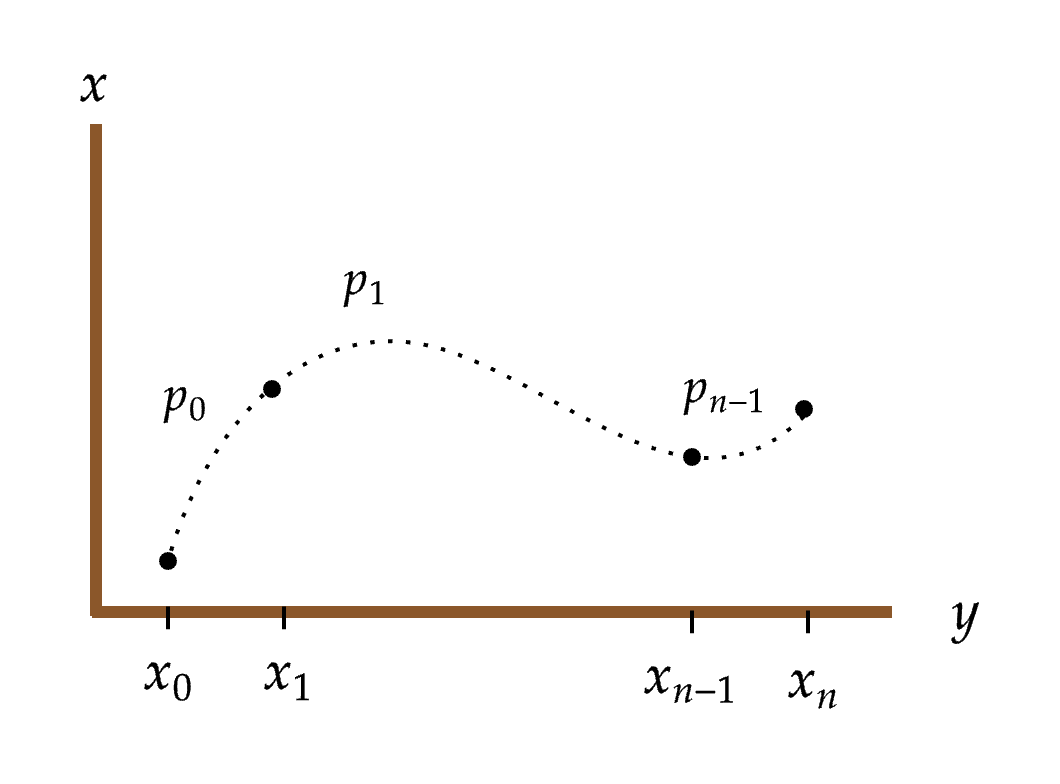
\includegraphics[width=\textwidth]{figures/fig-6.png}
    \end{center}
\end{marginfigure}

\noindent We will see three methods, each of which has a complexity in $\mathcal{O}(n)$, for spline interpolation. These are summarized in the table below,
\[
\begin{array}{|c|c|c|c|}
\hline \text { Spline Interpolant } & \text { Locality } & \text { Error } & \text { Smoothness }\\
\hline \hline \begin{array}{c}
\text { Piecewise } \\
\text { constant }
\end{array} & \begin{array}{c}
\text { Single } \\
\text {sub-intervals }
\end{array} & \mathcal{O}(h) & \begin{array}{c}
\text { Bounded } \\
\text { on } [a, b]  \\
\end{array} \\
\hline \begin{array}{c}
\text { Piecewise } \\
\text { linear }
\end{array} & \begin{array}{c}
\text { Two } \\
\text { sub-intervals }
\end{array} & \mathcal{O}(h^2) & C[a, b] \\
\hline \begin{array}{c}
\text { Piecewise } \\
\text { cubic }
\end{array} & \begin{array}{c}
\text { Neighboring } \\
\text { sub-intervals }
\end{array} & \mathcal{O}(h^4) & C^2[a, b] \\
\hline
\end{array}
\]

\LineBreak 

\noindent \textbf{Piece-wise constant splines} are defined as follows,
\begin{enumerate}
    \item $p_i(x) = a_i$ are polynomial of zeroth degree for $0 \leq i \leq n - 1$
    \item $S(x_n) = a_n$ so $n + 1$ unknowns need to be determined
\end{enumerate}
For each interval $\left[x_i, x_{i+1}\right)$ where $0 \leq i \leq n - 1$,
\[y_i=S\left(x_i\right)=p_i\left(x_i\right)=a_i \Rightarrow a_i=y_i\]
and the right-most endpoint is $a_n$. It follows that,
\[
S(x)= \begin{cases}y_i, & x \in\left[x_i, x_{i+1}\right) \\ y_n, & x=x_n\end{cases}
\]

\begin{rmk}
    The \textbf{local interpolation error} is,
    \[|f(x)-S(x)| \leq \frac{M_1}{1 !} \cdot \max _{x \in\left[x_{i-1}, x_i\right]}\left|x-x_{i-1}\right|=M_1 \cdot h_{i-1}\]
    since $S(x)$ is a polynomial of zeroth degree on each $\left[x_i, x_{i+1}\right)$. Letting $h:=\max _{1 \leq i \leq n} h_{i-1}$, the \textbf{global interpretation error} is,
    \[\max _{x \in[a, b]}|f(x)-S(x)| \leq \mathcal{O}(h)\]
\end{rmk}

\LineBreak

\noindent If \textbf{continuity} is an important feature for our model, then we can use a \textbf{linear polynomial} on each interval. That is, $p_i(x) := a_i+b_i\left(x-x_i\right)$ on the interval $[x_i, x_{i+1})$ for each $0 \leq i \leq n-1$. We impose,
\begin{enumerate}
    \item (Interpolation Condition) $y_i=S\left(x_i\right)=p_i\left(x_i\right)=a_i \Rightarrow a_i=y_i$ to ensure that our curve passes through our data points.
    \item (Continuity Condition) For $1 \leq i \leq n - 1$, we want $S\left(x_i^{-}\right)=S\left(x_i^{+}\right)$ at each $x_i$. Applying the definition of $p_i$, this implies that,
    \[y_{i-1}+b_{i-1}\left(x_i-x_{i-1}\right)=p_{i-1}\left(x_i\right)=S\left(x_i^{-}\right)=S\left(x_i^{+}\right)=p_i\left(x_i\right)=y_i\]
    which gives that,
    \[b_{i-1}=\frac{y_i-y_{i-1}}{x_i-x_{i-1}}=f\left[x_{i-1}, x_i\right]\]
    and at the right-most end-point,
    \[y_n=S\left(x_n\right)=p_{n-1}\left(x_n\right)=y_{n-1}+b_{n-1}\left(x_n-x_{n-1}\right)\]
\end{enumerate}
In summary, we have,
\[S(x)= \begin{cases}y_i+f\left[x_i, x_{i+1}\right]\left(x-x_i\right), & x \in\left[x_i, x_{i+1}\right) \\ y_{n-1}+f\left[x_{n-1}, x_n\right]\left(x-x_{n-1}\right), & x \in\left[x_{n-1}, x_n\right]\end{cases}\]
with the property that changes to $y_i$ will only affect $S(x)$ on the intervals $\left[x_{i-1}, x_i\right)$ and $\left[x_i, x_{i+1}\right)$. Our \textbf{error analysis} for piece-wise linear splines is similar to piece-wise constant splines.

\begin{marginfigure}
    \begin{center}
         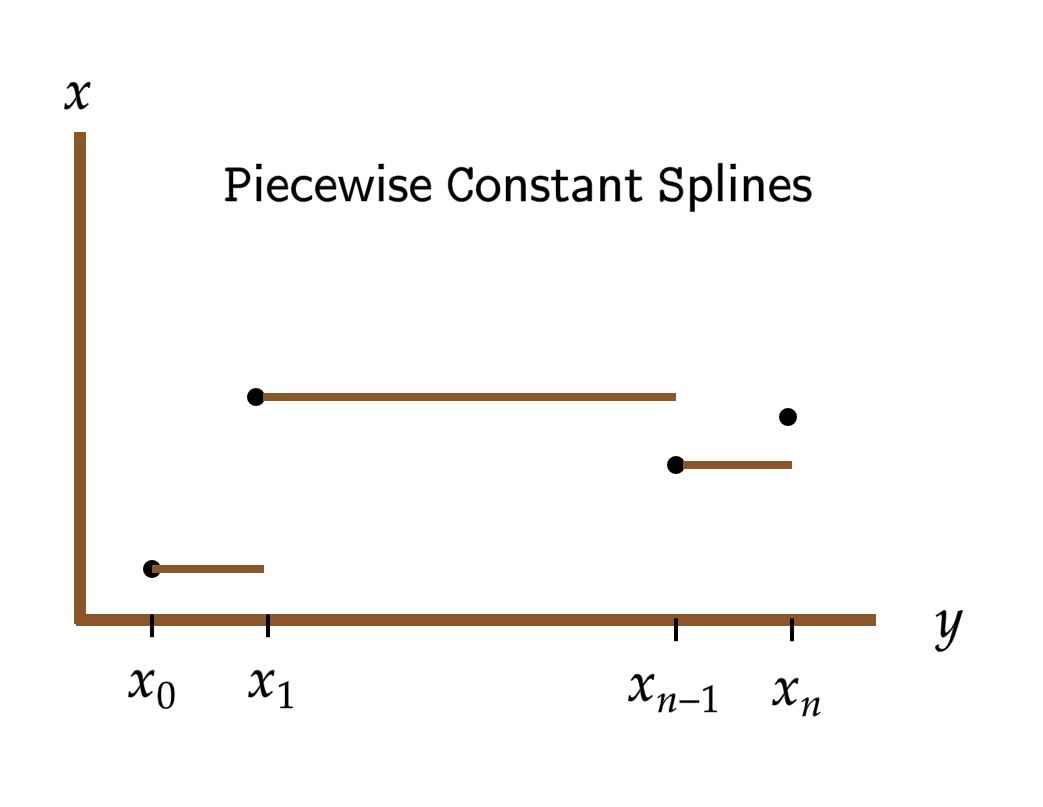
\includegraphics[width=\textwidth]{figures/fig-16.png}
    \end{center}
    \begin{center}
           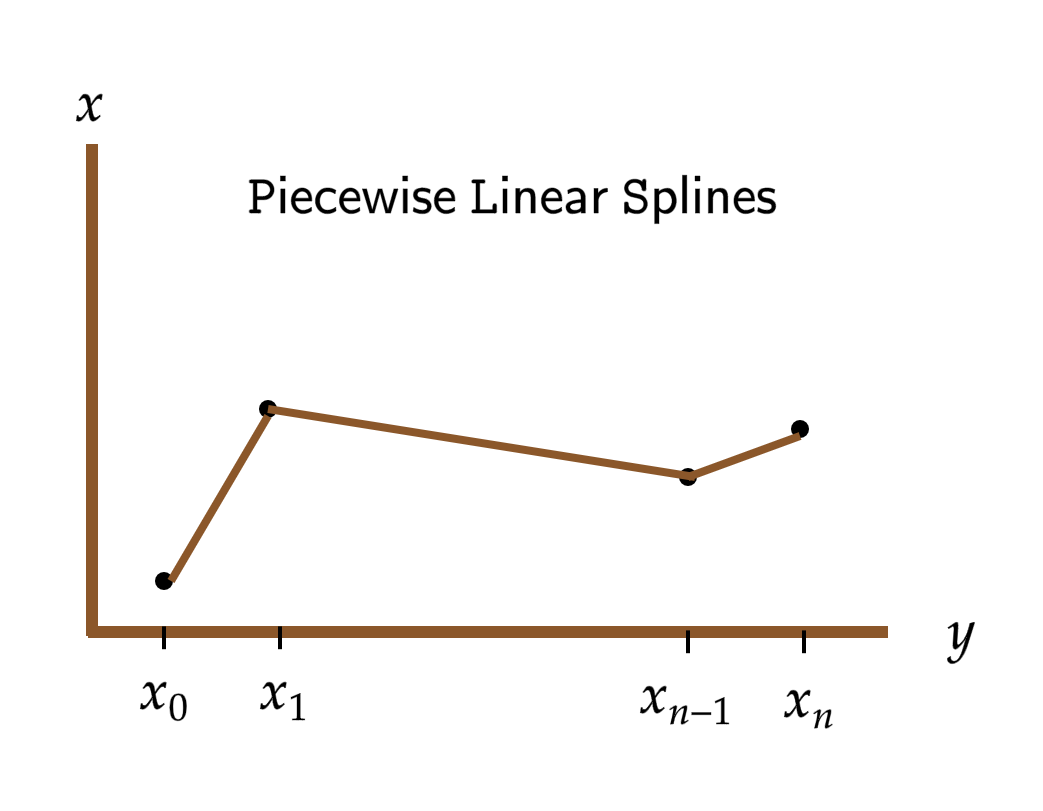
\includegraphics[width=\textwidth]{figures/fig-17.png}
    \end{center}
    \begin{center}
           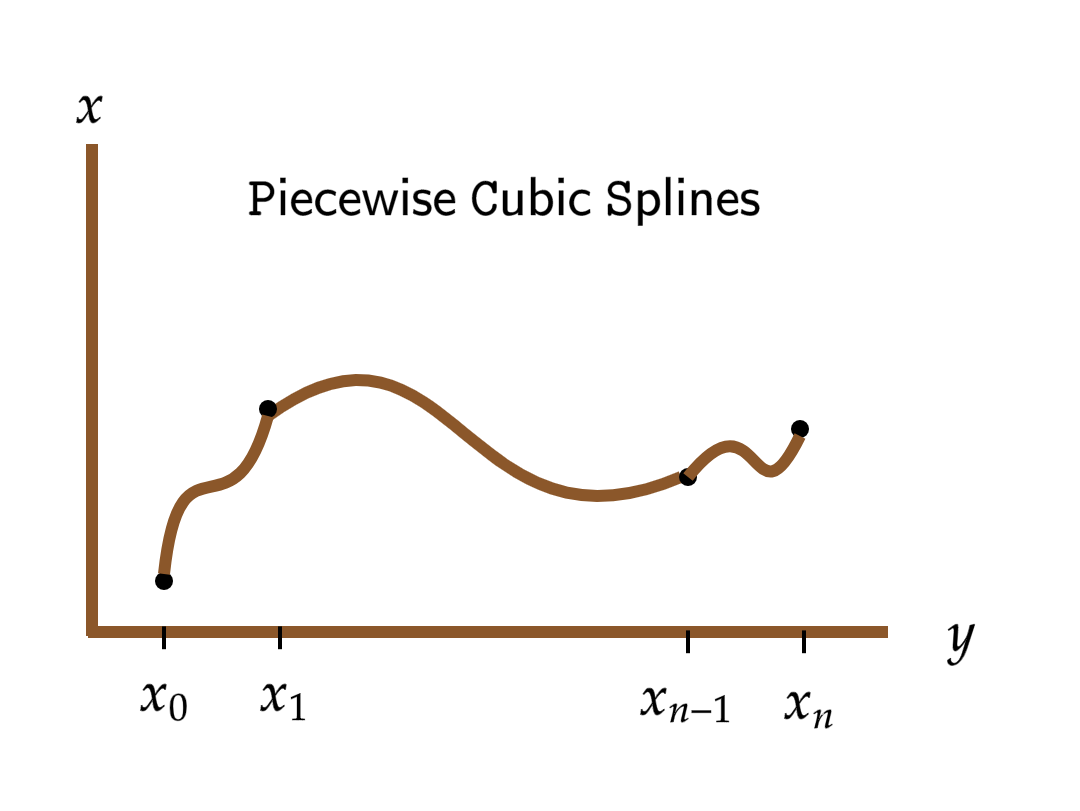
\includegraphics[width=\textwidth]{figures/fig-20.png}
    \end{center}
\end{marginfigure}

\begin{rmk}
     The \textbf{local interpolation error} is,
     \[|f(x)-S(x)| \leq \frac{M_2}{2 !} \underbrace{\max _{x \in\left[x_{i-1}, x_i\right]}\left|\left(x-x_{i-1}\right)\left(x-x_i\right)\right|}_{\texttt {maximized at midpoint}}=\frac{M_2}{8} h_{i-1}^2\]
     Letting $h:=\max _{1 \leq i \leq n} h_{i-1}$, the \textbf{global interpolation error} is,
     \[\max _{x \in[a, b]}|f(x)-S(x)| \leq \mathcal{O}(h^2)\]
\end{rmk}

\LineBreak

\noindent The drawback associated with piece-wise linear splines is that many applications require continuity in the first and second derivatives. This leads us to define \textbf{cubic piece-wise splines}. We will use a \textbf{cubic polynomial} on each interval. That is, $p_i(x)=a_i+b_i\left(x-x_i\right)+c_i\left(x-x_i\right)^2+d_i\left(x-x_i\right)^3$ for each $0 \leq i \leq n -1$. We impose,
\begin{enumerate}
    \item (Interpolation Condition) $y_i=S\left(x_i\right)=p_i\left(x_i\right)=a_i \Rightarrow a_i=y_i$ to ensure that the curve passes through our data points. We pick $y_n=S\left(x_n\right)=p_{n-1}\left(x_n\right)$ at the right-most end-point.
    \item (Continuity Condition \# A) For $1 \leq i \leq n-1$, $S\left(x_i^{-}\right)=S\left(x_i^{+}\right)$
    \item (Continuity Condition \# B) For $1 \leq i \leq n-1, S^{\prime}\left(x_i^{-}\right)=S^{\prime}\left(x_i^{+}\right)$
    \item (Continuity Condition \# C) For $1 \leq i \leq n-1, S^{\prime \prime}\left(x_i^{-}\right)=S^{\prime \prime}\left(x_i^{+}\right)$
\end{enumerate}
Conditions (2), (3), and (4) involve $n - 1$ equations, while (1) requires $n + 1$. In total, this is $4n-2$ equations with $4n$ unknowns. We require two more conditions to determine an interpolate uniquely:
\begin{enumerate}
    \item (Free Boundary Condition) We assume that,
    \[f^{\prime \prime}\left(x_0\right)=0 \quad \text{ and } \quad f^{\prime \prime}\left(x_n\right)=0\]
    \[\implies S^{\prime \prime}\left(x_0\right)=0 \text { and } S^{\prime \prime}\left(x_n\right)=0\]
    The resultant $S(x)$ is called the \textbf{natural spline}
    \item (Clamped Boundary Condition) We collect two additional data points $z_0$ and $z_n$ to specify the first derivative at the endpoints,
    \[S^{\prime}\left(x_0\right)=z_0 \quad \text { and } \quad  S^{\prime}\left(x_n\right)=z_n\]
    The resultant $S(x)$ is called the \textbf{complete spline}
    \item (Not-a-Knot Condition) We assume that,
    \[p_0^{\prime \prime \prime}\left(x_1\right)=p_1^{\prime \prime \prime}\left(x_1\right) \text { and } p_{n-2}^{\prime \prime \prime}\left(x_{n-1}\right)=p_{n-1}^{\prime \prime \prime}\left(x_{n-1}\right)\]
    The resultant $S(x)$ is called the \textbf{not-a-knot spline}
\end{enumerate}

\begin{marginfigure}
    The \textbf{not-a-knot} end condition means that, at the first and last interior break, even the third derivative is continuous (up to round-off error).
\end{marginfigure}

\noindent Given these different boundary conditions, we need to find the coefficients $a_i$, $b_i$, $c_i$, and $d_i$ to construct our polynomial. We write,
\begin{align*}
p_i(x) &=a_i+b_i\left(x-x_i\right)+c_i\left(x-x_i\right)^2+d_i\left(x-x_i\right)^3 \\
p_i^{\prime}(x) &=b_i+2 c_i\left(x-x_i\right)+3 d_i\left(x-x_i\right)^2 \\
p_i^{\prime \prime}(x) &=2 c_i+6 d_i\left(x-x_i\right)
\end{align*}
Recall that $h_i = x_{i+1} - x_i$ for $i \in [n-1]$ since our intervals are not uniformly spaced. The \textbf{interpolation condition} completely determines the constant terms $a_i$ since for all $n$ equations,
\[y_i=S\left(x_i\right)=p_i\left(x_i\right)=a_i \Rightarrow a_i=y_i\]
Plugging in $h_i$ and using our \textbf{right end-point condition},
\begin{align*}
y_n=S\left(x_n\right) &=p_{n-1}\left(x_n\right)=y_{n-1}+b_{n-1} h_{n-1}+c_{n-1} h_{n-1}^2+d_{n-1} h_{n-1}^3 \\
\Rightarrow f\left[x_{n-1}, x_n\right] &=b_{n-1}+c_{n-1} h_{n-1}+d_{n-1} h_{n-1}^2
\end{align*}
We will use \textbf{\# A} to obtain,
\begin{align*}
    &f\left[x_{i-1}, x_i\right]=b_{i-1}+c_{i-1} h_{i-1}+d_{i-1} h_{i-1}^2 \\
    &f\left[x_{n-1}, x_n\right]=b_{n-1}+c_{n-1} h_{n-1}+d_{n-1} h_n^2
\end{align*}
\textbf{\# B} to obtain,
\begin{align*}
    &b_i=b_{i-1}+2 c_{i-1} h_{i-1}+3 d_{i-1} h_{i-1}^2 \\
    &b_n=b_{n-1}+2 c_{n-1} h_{n-1}+3 d_{n-1} h_{n-1}^2
\end{align*}
and \textbf{\# C} to obtain,
\begin{align*}
&d_{i-1}=\frac{c_i-c_{i-1}}{3 h_{i-1}} \\
&d_{n-1}=\frac{c_n-c_{n-1}}{3 h_{n-1}}
\end{align*}
We have $4n$ equations with two additional auxiliary variables given by boundary conditions. It remains to solve $b_i$ in terms of $a_i$ and $c_i$. Substituting the expressions of $d_{i-1}$ into the equations for \textbf{\# B},
\[b_{i-1}=f\left[x_{i-1}, x_i\right]-\frac{h_{i-1}}{3}\left(c_i+2 c_{i-1}\right)\]
We can find equations for $c_i$ by substituting these expressions for $b_{i-1}$ and $d_{i-1}$ into the equations for \textbf{\# B}. Re-arranging the result,
\[h_{i-1} c_{i-1}+2\left(h_i+h_{i-1}\right) c_i+h_i c_{i+1}=3\left(f\left[x_i, x_{i+1}\right]-f\left[x_{i-1}, x_i\right]\right)\]
This is a \textbf{tridiagonal linear system} of $n - 1$ equations with $n - 1$ equations and $n + 1$ unknowns. The cubic spline boundary conditions will give the remaining two equations. In summary,

\begin{marginfigure}
    The system takes $\mathcal{O}(n)$ to solve.
\end{marginfigure}

\begin{ex}{Natural Cubic Spline}{label}
    We have $c_0 = 0 = c_n$, producing the $(n - 1) \times (n - 1)$ system,
    \[\mA \cdot \mathbf{c} = \mathbf{b}\]
    where $\mA$ is the matrix,
    \[
       \left(\begin{array}{cccc}
        2\left(h_0+h_1\right) & h_1 & & \\
        h_1 & 2\left(h_1+h_2\right) & & \\
        & \ddots & \ddots & \ddots \\
        & & 2\left(h_{n-3}+h_{n-2}\right) & h_{n-2} \\
        & & h_{n-2} & 2\left(h_{n-2}+h_{n-1}\right)
        \end{array}\right)
    \]
    and $\mathbf{c}$ and $\mathbf{b}$ are given by,
    \[
    \left(\begin{array}{c}
    c_1 \\
    c_2 \\
    \vdots \\
    c_{n-2} \\
    c_{n-1}
    \end{array}\right) \quad \quad \left(\begin{array}{c}
    3\left(f\left[x_1, x_2\right]-f\left[x_0, x_1\right]\right) \\
    3\left(f\left[x_2, x_3\right]-f\left[x_1, x_2\right]\right) \\
    \vdots \\
    3\left(f\left[x_{n-2}, x_{n-1}\right]-f\left[x_{n-1}, x_{n-2}\right]\right) \\
    3\left(f\left[x_{n-1}, x_n\right]-f\left[x_{n-2}, x_{n-1}\right]\right)
    \end{array}\right)
    \]
\end{ex}

\begin{ex}{Clamped Cubic Spline}{label}
    Combining equations for $c_i$ gives the $(n - 1) \times (n - 1)$ system,
    \[\mA \cdot \mathbf{c} = \mathbf{b}\]
    where $\mA$ is the matrix,
    \[
       \left(\begin{array}{ccccc}
        2 h_0 & h_0 & & & \\
        h_0 & 2\left(h_0+h_1\right) & h_1 & & \\
        & \ddots & \ddots & \ddots & \\
        & & h_{n-2} & 2\left(h_{n-2}+h_{n-1}\right) & h_{n-1} \\
        & & & h_{n-1} & 2 h_{n-1}
        \end{array}\right)
    \]
    and $\mathbf{c}$ and $\mathbf{b}$ are given by,
    \[
    \left(\begin{array}{c}
    c_1 \\
    c_2 \\
    \vdots \\
    c_{n-2} \\
    c_{n-1}
    \end{array}\right) \quad \quad \left(\begin{array}{c}
    3\left(f\left[x_0, x_1\right]-b_0\right) \\
    3\left(f\left[x_1, x_2\right]-f\left[x_0, x_1\right]\right) \\
    \vdots \\
    3\left(f\left[x_{n-1}, x_n\right]-f\left[x_{n-2}, x_{n-1}\right]\right) \\
    3\left(b_n-f\left[x_{n-1}, x_n\right]\right)
    \end{array}\right)
    \]
\end{ex}

\begin{rmk}
     Writing down the tridiagonal linear system for the \textbf{not-a-knot cubic} spline is left as an exercise. 
\end{rmk}

\noindent Since the $c_i$ coefficients are related through a linear system, a change in data for cubic splines is technically \textbf{non-local}. However, if only $y_i$ is changed, it can be shown that the largest change occurs at $c_i$, with changes in other $c_j$ decaying as a function of $|i - j|$. Thus, 
\[\max _{x \in[a, b]}|f(x)-S(x)| \leq C M_4 h^4=\mathcal{O}\left(h^4\right)\]
where $C > 0$ depends on the type of boundary conditions imposed.

\begin{marginfigure}
    The accuracy for cubic splines is comparable to Lagrange interpolation, but Runge's phenomenon is avoided on equally-spaced points.
\end{marginfigure}